\documentclass[11pt,oneside,letterpaper]{article}

% graphicx package, useful for including eps and pdf graphics
\usepackage{graphicx}
\DeclareGraphicsExtensions{.pdf,.png,.jpg}

% basic packages
\usepackage{color} 
\usepackage{parskip}
\usepackage{float}

% text layout
\usepackage{geometry}
\geometry{textwidth=15cm} % 15.25cm for single-space, 16.25cm for double-space
\geometry{textheight=22cm} % 22cm for single-space, 22.5cm for double-space

% helps to keep figures from being orphaned on a page by themselves
\renewcommand{\topfraction}{0.85}
\renewcommand{\textfraction}{0.1}

% bold the 'Figure #' in the caption and separate it with a period
% Captions will be left justified
\usepackage[labelfont=bf,labelsep=period,font=small]{caption}

% review layout with double-spacing
%\usepackage{setspace} 
%\doublespacing
%\captionsetup{labelfont=bf,labelsep=period,font=doublespacing}

% cite package, to clean up citations in the main text. Do not remove.
\usepackage{cite}
%\renewcommand\citeleft{(}
%\renewcommand\citeright{)}
%\renewcommand\citeform[1]{\textsl{#1}}

% Remove brackets from numbering in list of References
\renewcommand\refname{\large References}
\makeatletter
\renewcommand{\@biblabel}[1]{\quad#1.}
\makeatother

\usepackage{authblk}
\renewcommand\Authands{ \& }
\renewcommand\Authfont{\normalsize \bf}
\renewcommand\Affilfont{\small \normalfont}
\makeatletter
\renewcommand\AB@affilsepx{, \protect\Affilfont}
\makeatother

% comments
\usepackage{ulem}
\definecolor{purple}{rgb}{0.459,0.109,0.538}
\def\tb#1#2{\sout{#1} \textcolor{purple}{#2}} 
\def\tbc#1{\textcolor{purple}{[#1]}}

%%% TITLE %%%
\title{\vspace{1.0cm} \LARGE \bf Reassortment between influenza B lineages and the emergence of a co-adapted PB1-PB2-HA gene complex}

\author[1]{Gytis Dudas}
\author[2]{Trevor Bedford}
\author[1,3]{Samantha Lycett}
\author[1,4]{Andrew Rambaut}

\affil[1]{Institute of Evolutionary Biology, University of Edinburgh, Edinburgh, UK}
\affil[2]{Vaccine and Infectious Disease Division, Fred Hutchinson Cancer Research Center, Seattle, WA, USA}
\affil[3]{Institute of Biodiversity Animal Health and Comparative Medicine, University of Glasgow, Glasgow, UK}
\affil[4]{Fogarty International Center, National Institutes of Health, Bethesda, MD, USA}

\date{\today}

\begin{document}
\maketitle

\begin{abstract}

Influenza B viruses are increasingly being recognized as major contributors to morbidity attributed to seasonal influenza. 
Currently circulating influenza B isolates are known to belong to two antigenically distinct lineages referred to as B/Victoria and B/Yamagata lineages. 
Frequent reassortment between the segments of these two lineages has been noted in the past, but the effects of these reassortments have not been investigated in much detail.
\tbc{Expand abstract to broadly outline results and give a 1 sentence conclusion.}

\end{abstract}

\pagebreak

\section*{Introduction}
Seasonal influenza causes between 250,000 and 500,000 deaths annually and is comprised of three virus types (A, B and C) co-circulating in humans, of which influenza A is considered to cause the majority of seasonal morbidity and mortality \cite{flufactsheet}.
However, influenza B viruses are increasingly being recognized as important human pathogens \cite{paul-glezen2013}.
Following the 2009 A/H1N1 pandemic, influenza B has increased in prevalence and in the 2012/2013 European season as many as 53\% of influenza sentinel surveillance samples tested positive for influenza B \cite{ECDC1213}. 
Like other members of \textit{Orthomyxoviridae}, influenza B viruses have segmented genomes, which allow viruses co-infecting the same cell to exchange segments (a process known as reassortment). 
Influenza A viruses are widely considered to be a major threat to human health worldwide due to the ability to cause pandemics in humans via reassortment of circulating human strains and with non-human influenza A strains. 
Influenza B viruses are thought to primarily infect humans (and occasionaly seals \cite{osterhaus2000,bodewes2013} through a reverse zoonosis), and are thought to be unable to exhibit pandemics through the acquisition of antigenic novelty from an animal reservoir. 
Both influenza A and B evolve antigenically through time in a process known as antigenic drift, in which mutations to the haemagglutinin (HA) protein allow viruses to escape existing human immunity and persist in the human population, leading to recurrent seasonal epidemics \cite{bedford2013}.

Currently circulating influenza B viruses comprise two distinct lineages -- Victoria and Yamagata (referred to as Vic and Yam, respectively) -- named after strains B/Victoria/2/87 and B/Yamagata/16/88, that are thought to have genetically diverged in HA around 1983 \cite{rota1990}. 
These two lineages now possess antigenically distinct HA surface glycoproteins \tbc{CITE} allowing them to co-circulate in the human population.
Phylogenetic analysis of evolutionary rate, selective pressures and reassortment history of major clades of influenza B has shown extensive and often complicated patterns of reassortment between all segments of influenza B viruses between and within the Vic and Yam lineages \cite{chen2008}.
Here, we extend previous methods to reveal an evolutionarily intriguing pattern of reassortment in influenza B.
In our approach, membership to either the Victoria or Yamagata lineage in the tree of one segment is used to label the individual viruses in the tree of the other segments.
By modelling the transition between labels on a phylogenetic tree, reassortment events which result in the replacement of one segment's lineage by another show up as label changes along a branch (Figure \ref{methodFig}).
We use this method to reconstruct major reassortment events and quantify reassortment dynamics over time in influenza B viruses.

We show that despite extensive reassortment, three of the eight segments, PB1, PB2 and HA, still survive as distinct Victoria and Yamagata lineages, which appear to be co-adapted to the point where virions which do not contain PB1, PB2 or HA segments derived entirely from either the Vic or the Yam lineage have rarely been isolated and only circulate as transient lineages once isolated.
In other segments (PA, NP, NA, MP and NS) a single lineage has introgressed into the opposing background and been fixed in the influenza B population: Yam for PA, NP, NA and MP and Vic for NS.
This has occured through repeated reassortments and subsequent fixation of reassortant viruses within the influenza B population.

\begin{figure}[h]
 \centering		
	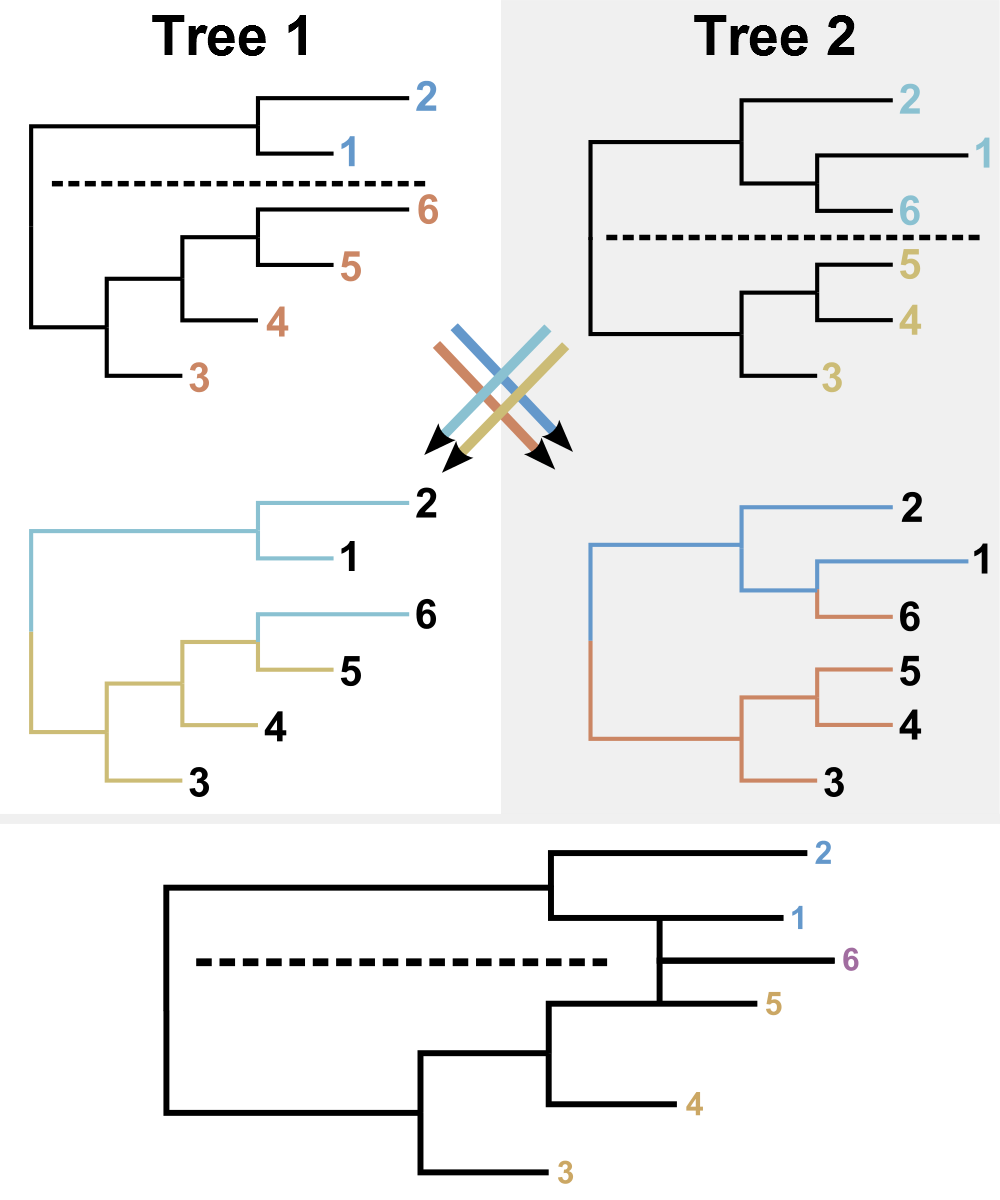
\includegraphics[width=0.45\textwidth]{figures/TreeFigure2}
	\caption{\textbf{Schematic analysis of reassortment patterns.}
	A) We begin by assigning sequences falling on either side of a specified bifurcation within each segment tree to different lineages, in this case, the Victoria and Yamagata bifurcation that occurred in the early 1980s.
	B) We then transfer lineage labels from one tree to the same tips in another tree.
	Label switches thus indicate reassortment events that combine lineages falling on different sides of the Vic/Yam bifurcation.
	C) A reassortment graph depiction shows that tip number 6 is determined to be a reassortant.
	\tbc{Relabel as "Segment 1" and "Segment 2" instead of "Tree 1" and "Tree 2".}
	}
	\label{methodFig}
\end{figure}

\section*{Methods}

\subsection*{Sequences and lineage assignment}

We compiled a dataset of 452 complete influenza B genomes from GISAID \cite{GISAID} dating from 1984 to 2012 (accession numbers and laboratory acknowledgements can be found in supplementary information). 
The segments of each strain were assigned to a lineage (either Vic or Yam) by making maximum likelihood trees of each segment \tbc{using what software?} and identifying whether the isolate was more closely related to B/Victoria/2/87 or B/Yamagata/16/88 sequences in that segment, with the exception of the NS segment (B/Victoria/2/87 was a reassortant and possessed a Yam lineage NS \cite{lindstrom1999}), where B/Czechoslovakia/69/1990 was considered as being representative of Victoria lineage.

Each strain was thus assigned 8 lineages depending on the combination of lineages it belongs to in all trees (for example all segments except for NS in strain B/Victoria/2/87 belong to Vic lineage and can thus be represented as V,V,V,V,V,V,V,Y). 

\subsection*{Building trees}
Temporally-calibrated phylogenies were recovered for each segment using the Markov chain Monte Carlo (MCMC) methods in the BEAST software package \cite{drummond2012}.
Here, we modeled the substitution process using the HKY model of nucleotide substitution, with separate transition models for each of the 3 codon partitions, and additionally estimate realized synonymous and non-synonymous substitution counts \cite{obrien2009}.
We used a flexible Bayesian skyride demographic model \cite{minin2008}.
We accounted for incomplete sampling dates for 94 sequences (of which 93 only had year of isolation and 1 had only year and month of isolation) whereby tip date is estimated as a latent variable in the MCMC integration.
We ran 3 independent MCMC chains, each with 200 million states, sampled every 20,000 steps and discarded the first 10\% of the MCMC states as burn-in.
After assessing convergence of all 3 MCMC chains by visual inspection using Tracer \tbc{CITE}, we combined samples across chains to give a total of 27,000 samples from the posterior distribution of trees.
\tbc{The MCC tree for each segment should be shown in supplemental information.  I would imagine one figure with eight panels.}

Every sequence was assigned 7 discrete traits corresponding to the lineages of all other segments with which a strain was isolated (e.g. PB1 tree had PB2, PA, HA, NP, NA, MP and NS as traits and V or Y as trait values).
We inferred the ancestral state of lineages in each segment by modelling transitions between these discrete traits using an asymmetric transition matrix \tbc{CITE asymmetric model} with Bayesian stochastic search variable selection (BSSVS) to estimate significant rates \cite{lemey2009}). Because the posterior set of trees for a single segment has branches labelled with the inferred lineage in the remaining 7 segments, we can detect inter-lineage reassortments between pairs of segments by observing trait transitions, i.e. Yam to Vic or Vic to Yam (see Figure \ref{methodFig}). 
In addition, by reconstructing the ancestral state of all other genomic segments jointly we can infer co-reassortment events when more than one trait transition occurs on the same node in a tree.

\subsection*{Measures of diversity}
We inferred the diversity of each segment at a single point in time by estimating the date of the most recent common ancestor of all branches at yearly intervals, which places an upper bound on the maximum amount of diversity existing at each time period.
In addition, we calculated mean pairwise TMRCA between branches labelled as Vic and Yam for PB1, PB2 and HA.
This gave us a measure of how much a particular segment reassorts with respect to PB1, PB2 and HA segments.
If Vic and Yam lineages of PB1, PB2 and HA segments were to be considered as being separate populations this measure would be equivalent to `between population' diversity.

We also calculated the total amount of evolutionary time spent by each segment with entirely Vic, entirely Yam or mixed lineage PB1, PB2 and HA segments.
We do this by summing the branch lengths in each tree under 3 different lineage combinations of the PB1, PB2 and HA segments: PB1-PB2-HA derived entirely from Yamagata lineage, PB1-PB2-HA entirely derived from Victoria lineage and PB1-PB2-HA derived from a mixture of the two lineages.
This gives a measure of how successful, over long periods of time, each particular PB1-PB2-HA constellation has been.

\subsection*{Tree to tree similarities}
We subsampled our combined posterior distribution of trees to give a total of 2700 trees.
Pairwise comparison between each pair of segments was performed by comparing individual pairs of sampled trees.

We express the similarity of two trees by referring to the mean of the distribution of TMRCA differences ($\Delta$TMRCA) between pairs of tips in the two trees.
These parameters are estimated for each pairing of trees at each MCMC state and provides us with 95\% highest posterior density intervals for those parameters, thus giving us the ability to test specific hypotheses regarding similarities between the trees of different segments.
Our approach exploits the branch scaling used by BEAST \cite{drummond2012}, since the trees are scaled in absolute time and insensitive to variation in nucleotide substitution rates between segments, allowing for direct comparisons between TMRCAs in different trees.

If we are comparing TMRCAs of the same two tips in tree A and tree B we express it as 
\begin{equation}
\frac{[A_{i}:A_{i}']+[B_{i}:B_{i}']}{2\times [A_{i}:B_{i}]},
\frac{[A_{i}:A_{i}']+[B_{i}:B_{i}']}{2\times [A_{i}:B_{i}]},
\end{equation}
where $f(A_i,B_j)$ is the $\Delta$TMRCA of a pair of tips between the \textit{i}th tree derived from alignment A and the \textit{j}th tree derived from alignment B and $f(A_i,A_j)$ is the $\Delta$TMRCA between the same pair of tips between \textit{i}th tree derived from alignment A and \textit{j}th tree derived from an independent run of alignment A, to control for variability in tree topology stability over the course of the MCMC chain caused by differences in alignment lengths used to produce the trees.

Subtree prune and regraft (SPR) distances between phylogenetic trees are an approximate measure of the numbers of reassortment or recombination events.
Exact SPR distances are difficult to compute, as they depend on the SPR distance itself and are impractical to compute for posterior distributions of trees except for the most similar trees.
We calculated approximate SPR distances \cite{whidden2009,whidden2010,whidden2013} to quantify the numbers of reassortments that have taken place between all pairs of segments.
Approximate SPR distances were normalized using the procedure described above.

\subsection*{Estimating linkage disequilibrium across the influenza B genome}
We attempted to estimate linkage disequilibrium (LD) between amino acid sites across the longest proteins encoded by each segment of the influenza B virus genome.
We use the $\chi^{2}_{df}$ statistic \cite{zhao2005} for quantifying LD, as it is equal to the widely used \textit{r$^{2}$} LD statistic at biallelic loci, but also quantifies LD when there are more than two alleles per locus.
LD was estimated only at loci where each `allele' was represented by at least two isolates.
We ignored gaps in the alignment and did not consider them as polymorphisms.
However, there is at least one polymorphic indel within the HA protein, which is associated with the Vic-Yam split and not with incomplete sequences.

We also calculated mean LD for all pairs of segments to quantify the overall association between them.

\subsection*{Confirming findings with a larger dataset through lineage assignment}
The sequences of all 1433 available sequences of PB1, PB2, HA and NA segments from the same isolates sampled 1984-2013 were compiled from GISAID.
Neighbor-joining trees \cite{saitou1987} of PB1, PB2 and HA segments were made and each sequence assigned to a lineage based on grouping with either B/Victoria/2/87 or B/Yamagata/16/88 sequences.
Isolates which were not assigned entirely to either the Vic or the Yam lineage across PB1, PB2 and HA segments were extracted and identified as PB1-PB2-HA reassortants.

\section*{Results}

\subsection*{PA, NP, NA, MP and NS segments have periodically lost diversity}

The split of Vic and Yam lineages can be seen in all segments \cite{chen2008}.
Following the split of the two lineages, each segment could be assigned to either Vic or Yam lineage and inter-lineage reassortment events have yielded mixed-lineage genome constellations.
Some viruses with mixed-lineage genomes have become fixed in the influenza B virus population \textit{i.e.} became the `trunk' of the phylogenetic tree of a segment.

We find that Vic lineage PA, NP, NA and MP segments have gone extinct (\textit{i.e.} no Vic lineage sequences of those segments have been sampled in recent years see Figure \ref{lineageRatiosOverTime}), replaced entirely by the respective segments of Yam lineage in viruses bearing a Vic lineage HA.
Conversely, Vic lineage NS has become fixed in the influenza B virus population as well.
By looking at the most recent common ancestor of all lineages existing at yearly timeslices within the tree of each segment (see Figure \ref{tmrcaOT}), it is clear that PA, NP, NA, MP and NS segments have undergone periodic losses of diversity, whereby all sequences sampled more recently trace their ancestry to increasingly more recent common ancestors.


\subsection*{PB1, PB2 and HA segments continue to circulate as two lineages}
We find that PB1, PB2 and HA segments of influenza B have not undergone lineage turnover, unlike PA, NP, NA, MP and NS segments.
This is shown in Figure \ref{tmrcaOT}, where PB1, PB2 and HA lineages are shown to be derived from a consistently old TMRCA, indicating continued accumulation of diversity since the split of Vic and Yam lineages.
We suggest that the maintenance of both Vic and Yam lineages in PB1, PB2 and HA segments might be caused by the action of some form of balancing selection.
In Figure \ref{lineageRatiosOverTime} the ratios at which Vic and Yam lineages of PB1, PB2 and HA segments have been isolated appear to be close to 0.5 over long periods of time.
On a year-to-year basis the ratios can fluctuate dramatically suggesting frequency-dependent domination of one or the other lineage within a given year.

\subsection*{PB1, PB2 and HA segments do not reassort across the Victoria-Yamagata boundary}
By measuring mean pairwise diversity between branches in each tree that were assigned either a Vic or Yam label in other segments, we look for reductions in diversity, which indicate that an inter-lineage reassortment event has taken place.
Because we are taking the mean of pairwise comparisons, this method gives a qualitative measure of panmixis between Victoria and Yamagata lineages in two trees.

We focus only on PB1, PB2 and HA lineage labels, since all other segments have fixed either the Vic or the Yam lineage.
Increasing mean between label TMRCAs for all segments in Figure \ref{betweenDiversity} indicate that every segment has reassorted with respect to Victoria and Yamagata lineages of PB1, PB2 and HA segments.
However, we also see that PB1, PB2 and HA labels show reciprocal preservation of diversity after 1997.
This suggests that no reassortment events have taken place between Victoria and Yamagata lineages of PB1, PB2 and HA segments (\textit{i.e.} PB1, PB2 and HA traits after 1997 only `meet' at the root of PB1, PB2 and HA trees).
In a time period close to the initial split of Vic and Yam lineages (1986--1996) we see reduced diversity between Vic and Yam labels of PB1 and PB2 segments on one hand and HA on the other.
These reductions in diversity represent small clades with PB1 and PB2 segments from one lineage and the HA segment from another, which go extinct by 1997.

In addition, the assignment of Vic or Yam lineages of PB1, PB2 and HA segments to branches of other segment trees is very similar and often identical.
This results in PB1, PB2 and HA lineage labels switching between Vic and Yam simultaneously in all trees after 1997, suggesting co-reassortment of Vic and Yam lineages of PB1, PB2 and HA segments. 

\begin{figure}[h]
	\centering		
	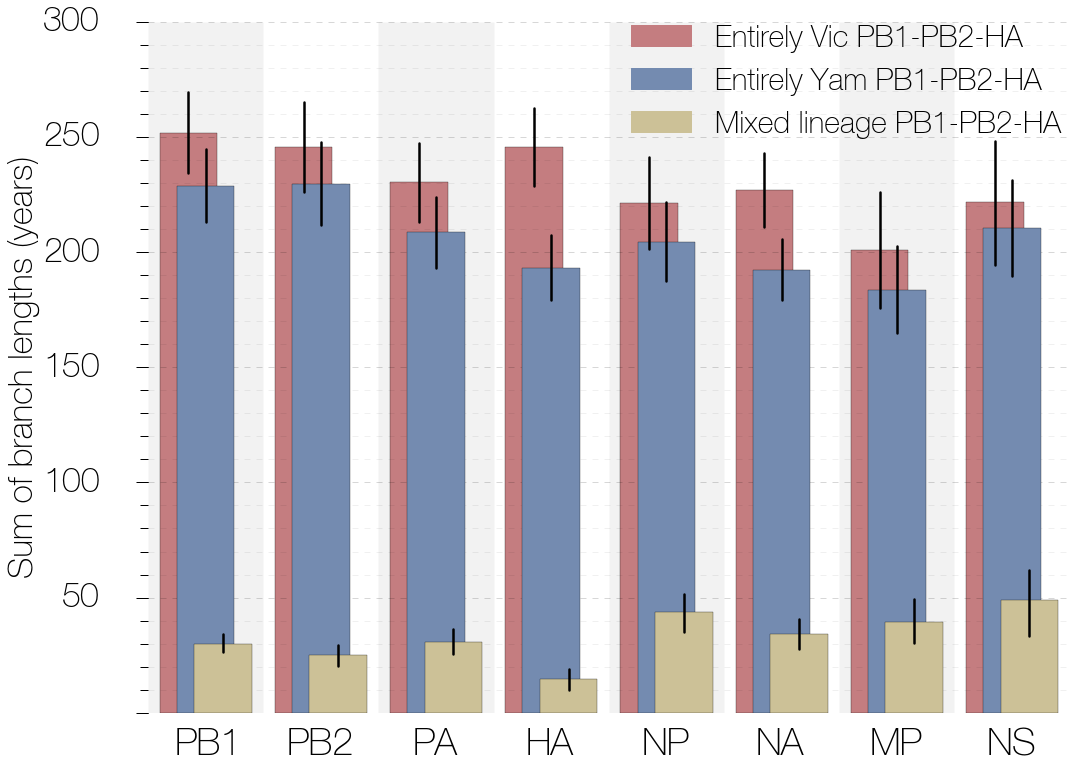
\includegraphics[width=0.95\textwidth]{figures/InfB_stateTime.png}
	\caption{\textbf{Amount of evolutionary time spent under different PB1-PB2-HA constellations.}
All segments have spent significantly more of their history with entirely Vic or entirely Yam-derived PB1-PB2-HA complexes.
All horizontal lines indicating uncertainty are 95\% highest posterior densities (HPDs).}
	\label{stateTime}
\end{figure}


\subsection*{Recent PB1-PB2-HA constellations are entirely derived from Victoria or Yamagata lineage segments}
\tbc{Can you reject the hypothesis that PB1 and PB2 stuck to HA stochastically?}

We find that PB1, PB2 and HA segments, in addition to not reassorting across the Vic-Yam lineage boundary since 1997, form co-reassorting segment complexes derived entirely of Vic or Yam lineage segments.
Figure \ref{stateTime} shows the sum of branch lengths which were labelled as having entirely Vic, entirely Yam or mixed-lineage PB1, PB2 and HA segments.
Due to lack of reassortment between Vic and Yam lineages of PB1, PB2 and HA (Figure \ref{betweenDiversity}) all segments have spent significantly longer periods of evolutionary time with either entirely Vic-derived or entirely Yam-derived than with mixed-lineage PB1, PB2 and HA constellations (Figure \ref{stateTime}).

We have identified 3 instances of mixed-lineage PB1-PB2-HA reassortants from the data with the following PB1-PB2-HA constellations: VVY (B/Bankok/163/1990-like, 13 sequences isolated 1990 -- 5 Jan 1995), YVV (B/Nanchang/630/1994-like, 2 sequences isolated 1994 -- 1996) and YVY (B/New York/24/1993-like, 2 sequences isolated 8 Jan 1993 -- 1994).
An additional instance of reassortants with a YYV PB1-PB2-HA constellation (B/Waikato/6/2005-like, 16 sequences isolated June 9 -- November 12 in 2005) was discovered when investigating a larger dataset with only PB1, PB2, HA and NA sequences.
In all cases, PB1-PB2-HA reassortants have not persisted for prolonged periods of time and have not been fixed in the influenza B population.
In particular reassortment events combining PB1 and PB2 segments of different lineages, \textit{e.g.} B/Nanchang/630/1994-like and B/New York/24/1993-like isolates (each having two sequences), exhibit poor sampling and short circulation times (up to two years in the case of B/Nanchang/630/1994-like viruses).
In contrast, reassortments combining PB1+2 and HA of different lineages (B/Bankok/163/1990-like and B/Waikato/6/2005-like isolates) have more isolates and circulated for much longer periods of time in the past (up to 4 years for B/Bankok/163/1990-like, although B/Waikato/6/2005-like only circulated for 5 months).

\begin{figure}[h]
	\centering		
	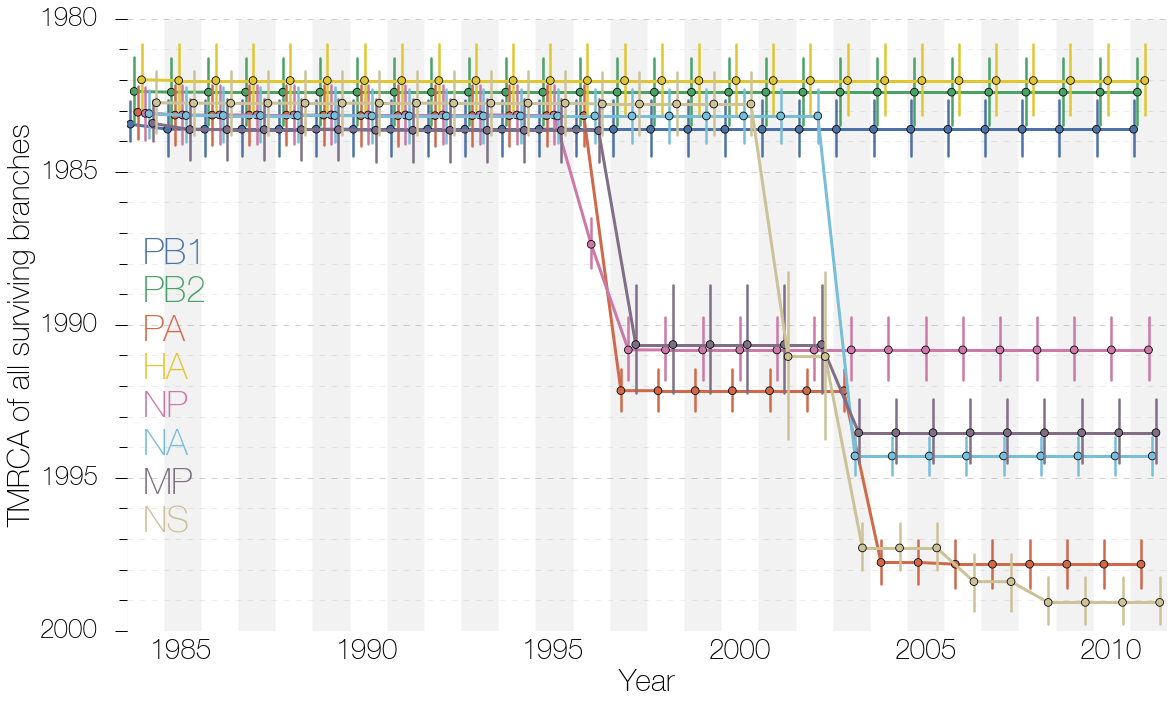
\includegraphics[width=0.95\textwidth]{figures/InfB_tmrcaOT_lines.png}
	\caption{\textbf{Oldest TMRCA of all surviving lineages over time.}
PA, NP, NA, MP and NS segments of influenza B viruses show periodic losses of diversity, indicating lineage turn over.
PB1, PB2 and HA segments, on the other hand, maintain the diversity dating back to the initial split of Vic and Yam lineages.
All vertical lines indicating uncertainty are 95\% highest posterior densities (HPDs).}
	\label{tmrcaOT}
\end{figure}

(comment - need higher resolution for lineage ratios figure or switch to vector graphics)
\begin{figure}[h]
	\centering	
	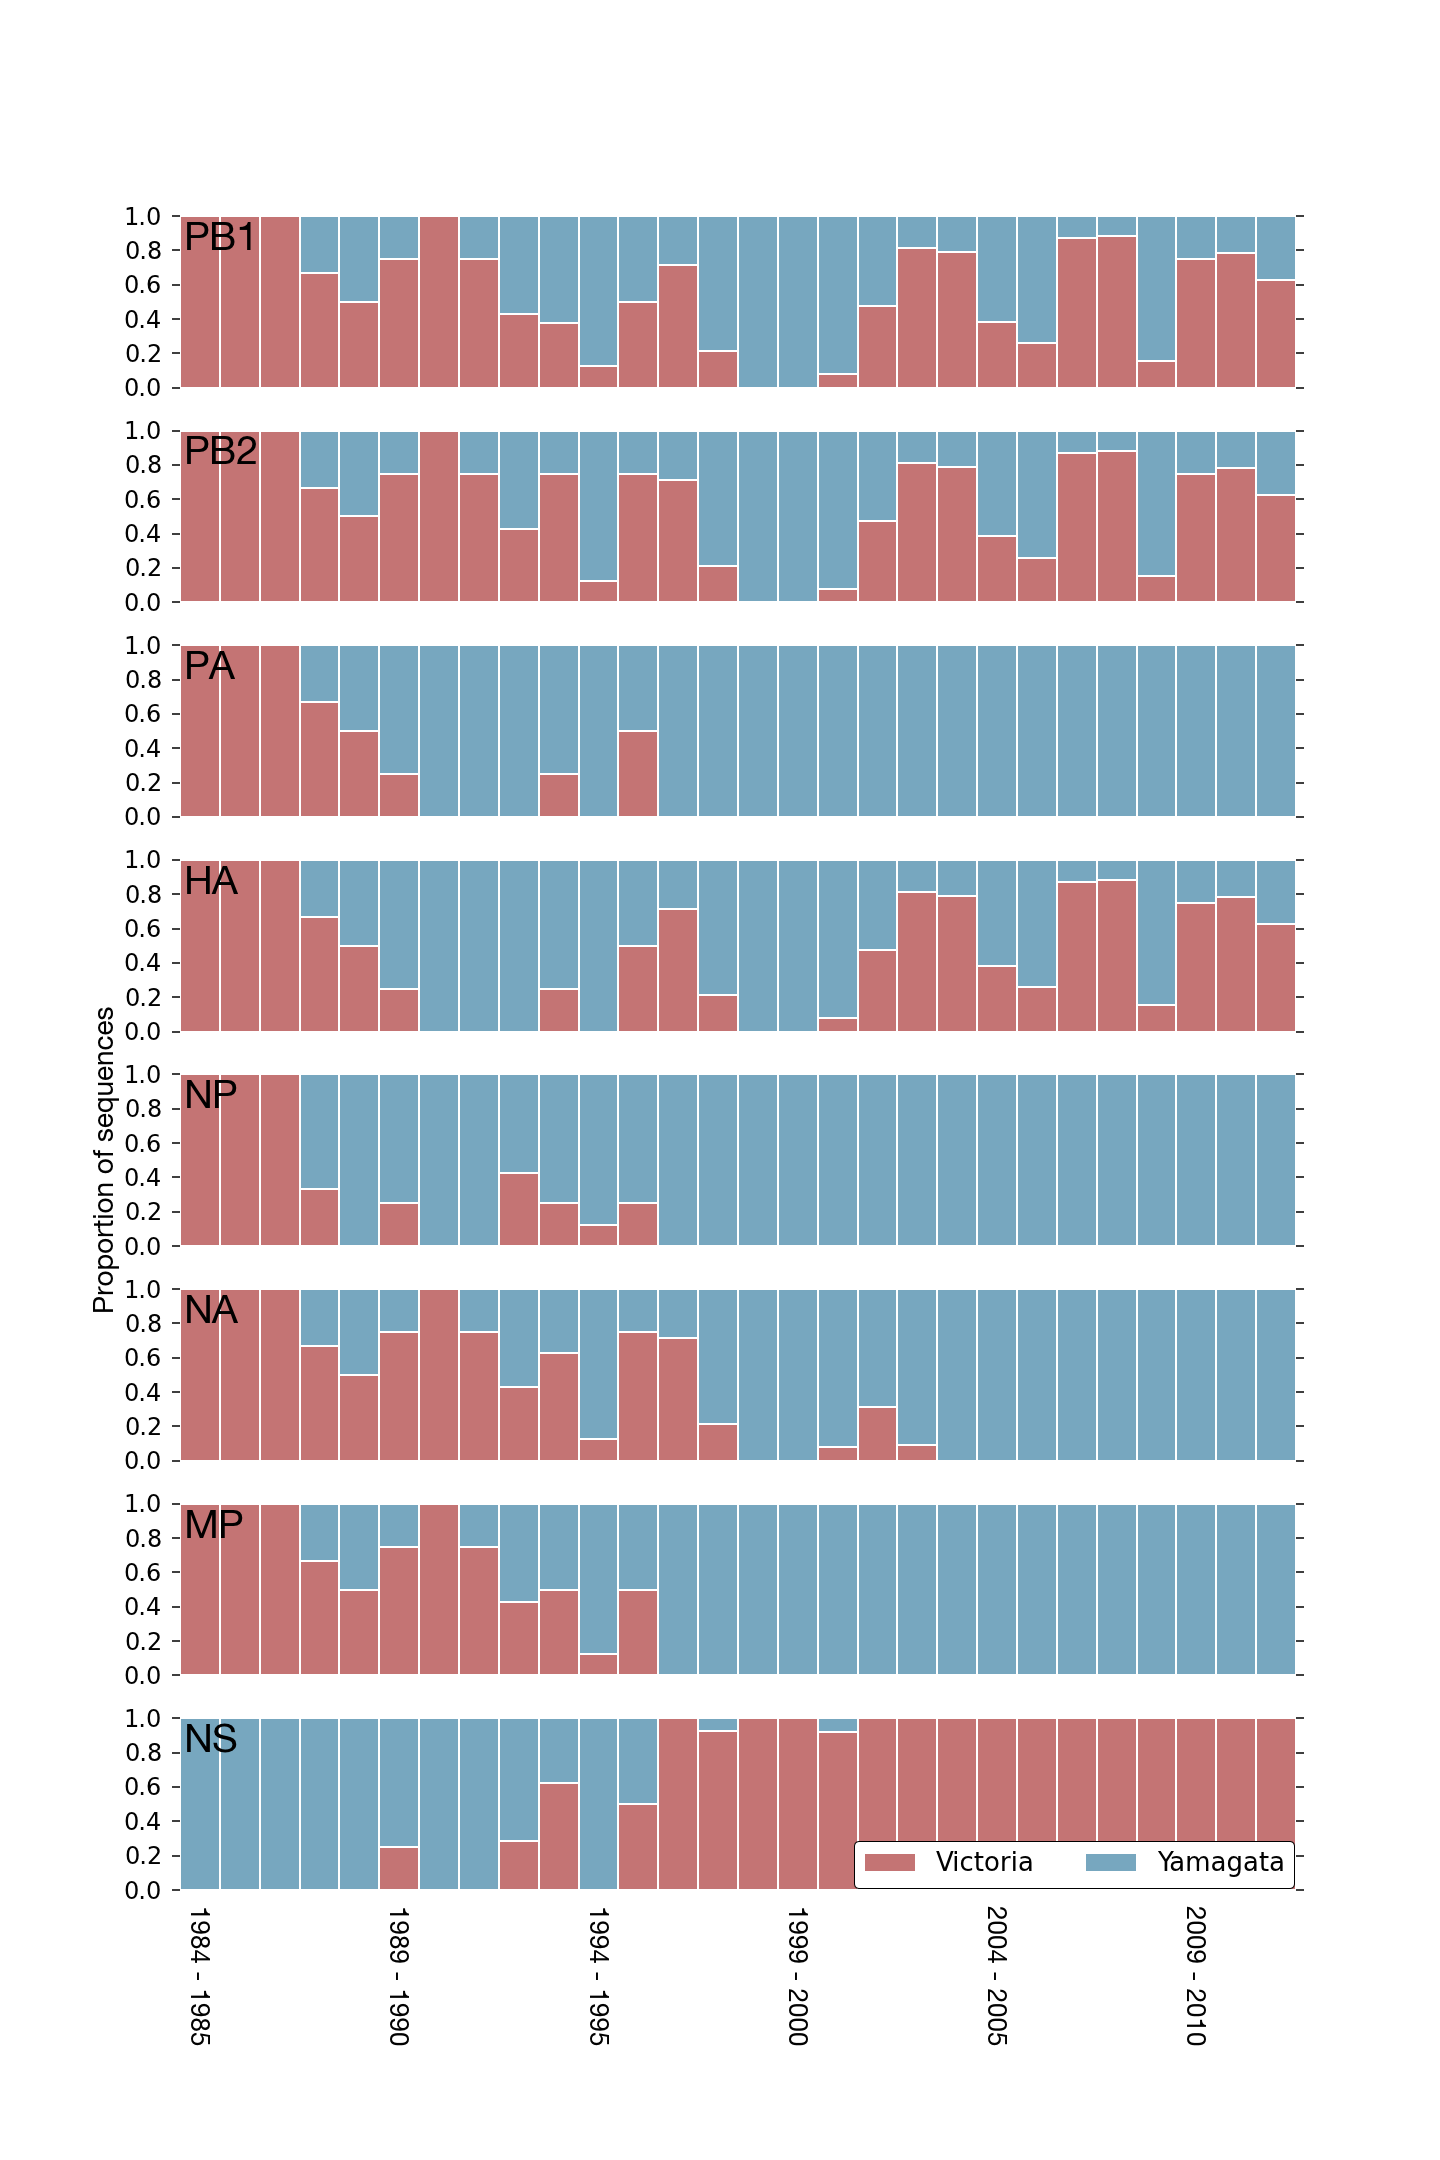
\includegraphics[width=0.75\textwidth]	{figures/InfB_LineageRatiosOverTime.png}
	\caption{\textbf{Ratio of lineages in the dataset.}}
	\label{lineageRatiosOverTime}
\end{figure}

\begin{figure}
	\centering		
	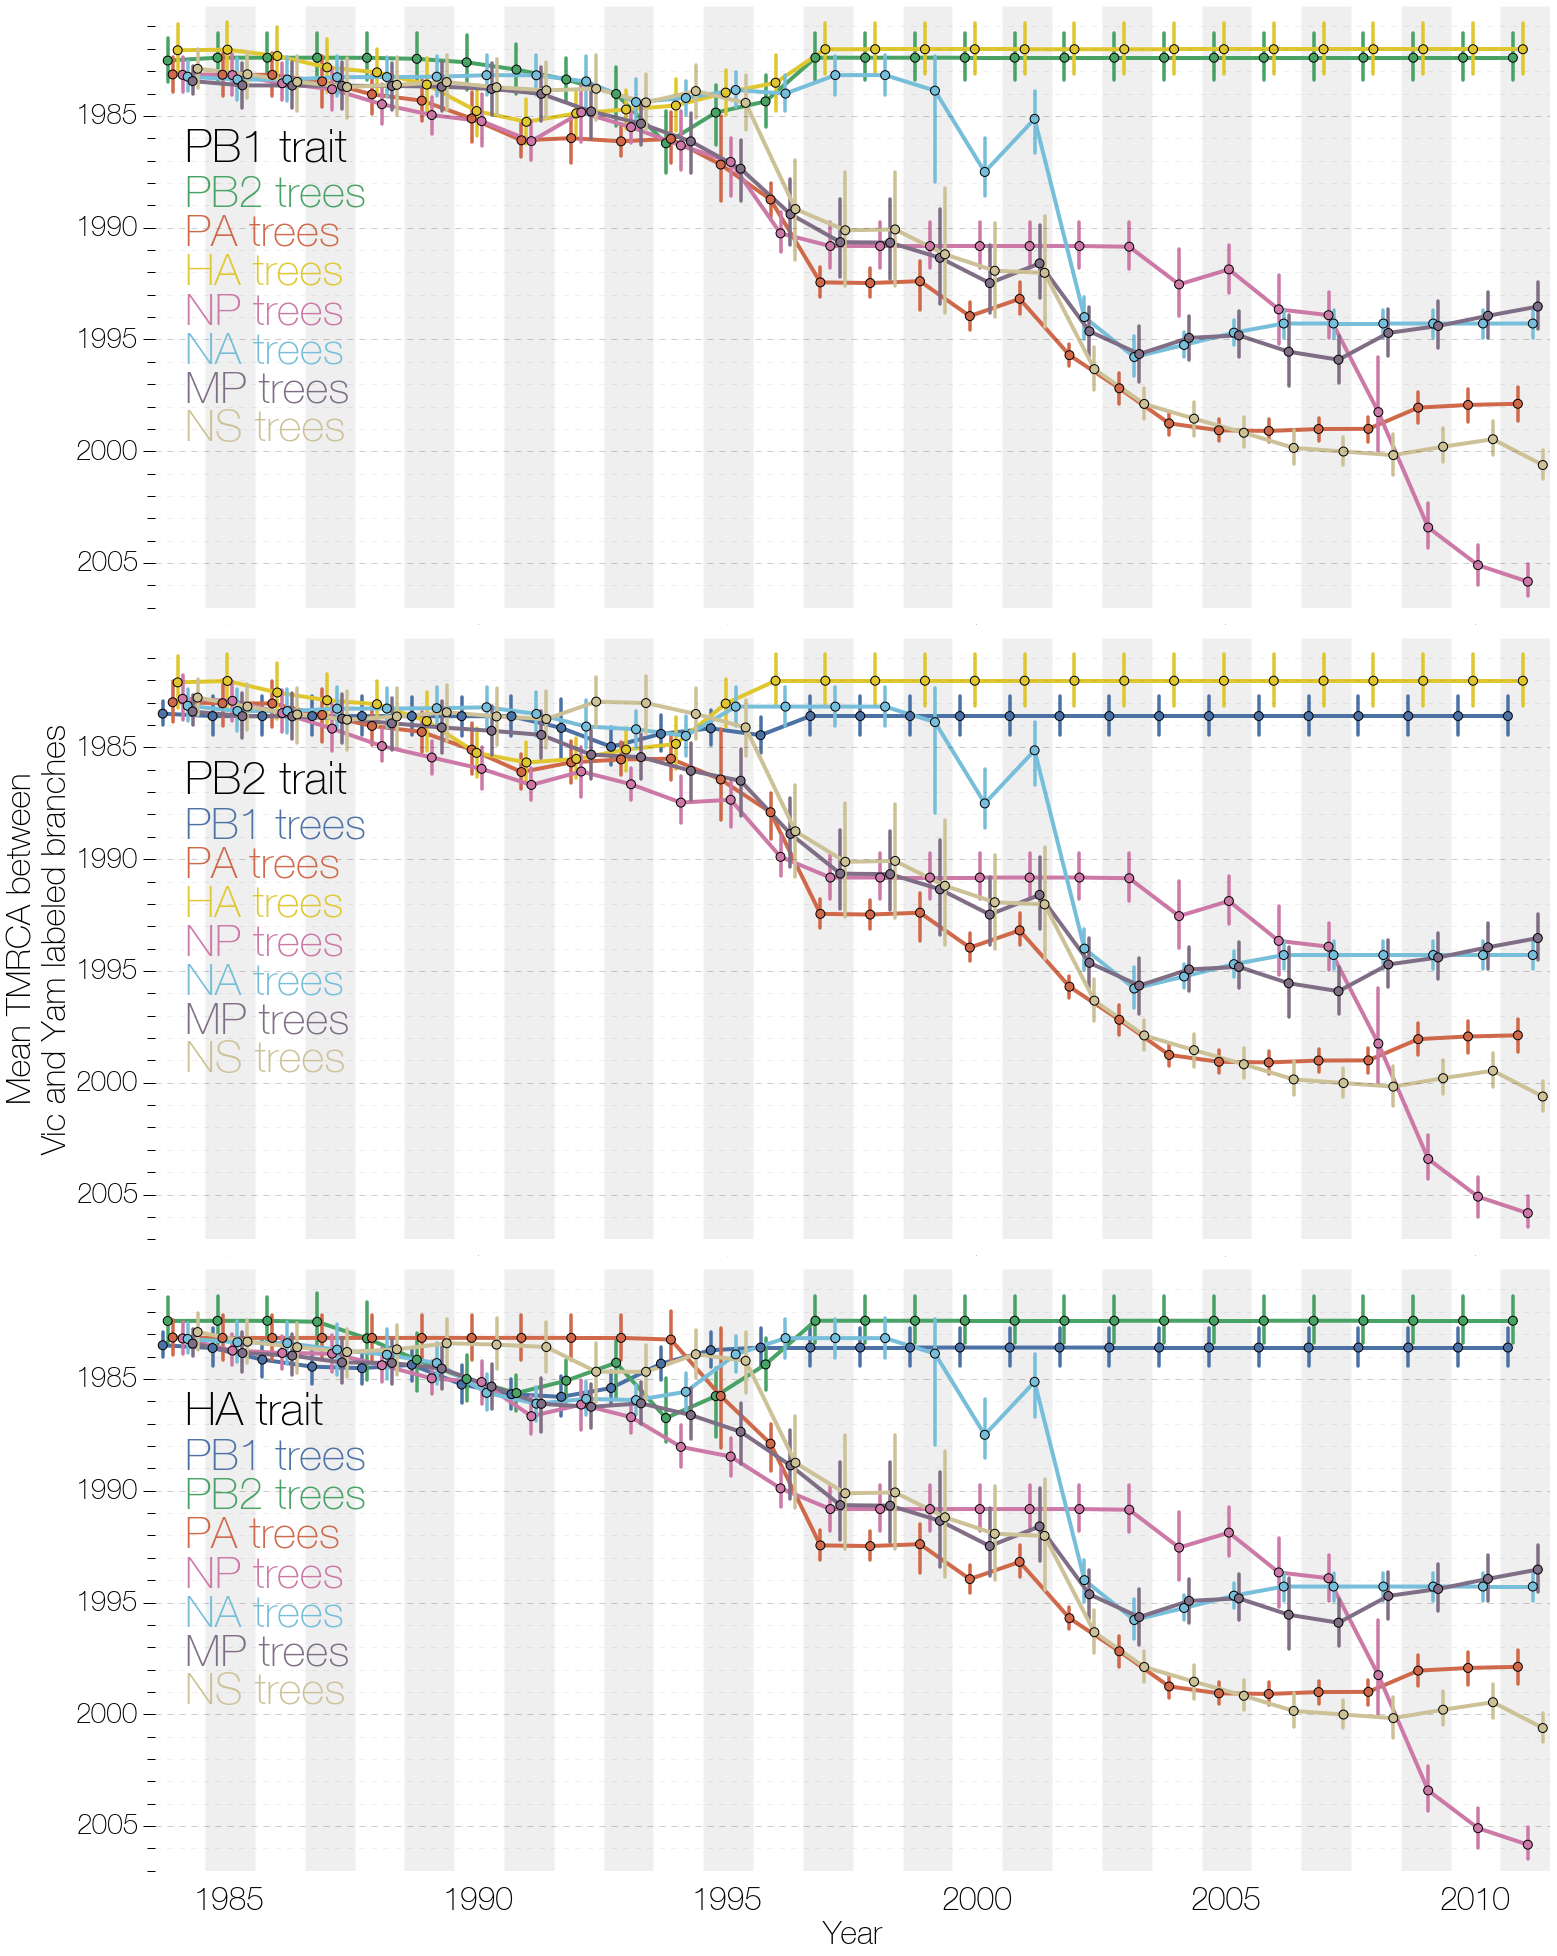
\includegraphics[width=0.95\textwidth]{figures/InfB_betweenDiversity.png}
	\caption{\textbf{Mean pairwise TMRCA between Vic and Yam branches under PB1, PB2 and HA label sets.}
PB1, PB2 and HA segment labels indicate that these segments show reciprocal preservation of diversity, which dates back to the split of Vic and Yam lineages.
All other segments show increasingly more recent TMRCAs between branches labelled as Vic and Yam in PB1, PB2 and HA label sets.
All vertical lines indicating uncertainty are 95\% highest posterior densities (HPDs).}
	\label{betweenDiversity}
\end{figure}

\subsection*{Railroad schematic plot of influenza B reassortment history}

\tbc{Are the observed rates of extinction / co-option fit with the effective population of the flu B population?  I.e. we generally get 10 years back to a common ancestor within a lineage / segment.  Can we think of the extinction of segments as an aspect of there existing a loosely panmictic flu B population for everything but PB1, PB2 and HA?}

We reconstructed reassortment events that were detected by using lineage labels.
Figure \ref{railroadPlot} focuses only on reassortments that have occured after 1990.
We identify 5 major reassortant genome constellations (given in order PB1-PB2-PA-HA-NP-NA-MP-NS) circulating 1992 -- 2011: B/Alaska/12/1996-like (YYYYYYYV), B/Nanchang/2/1997-like (VVYVYVYV), B/Iowa/03/2002-like (VVYVYYYV), B/California/NHRC0001/2006-like (VVYVYYYV) and B/Brisbane/33/2008-like (VVYVYYYV).
Figure \ref{railroadPlot} shows that reassorting segments appear to evolve with a considerable degree of autonomy.
For example, the NP lineage that entered a largely Victoria lineage derived genome and gave rise to the B/Nanchang/2/1997-like isolates continued circulating until 2010, even though other segments it reassorted with in 1995 -- 1996 (PA and MP) went extinct following the reassortments that led to B/Iowa/03/2002-like isolates.
A more extreme example is the NS segment, which in B/Iowa/03/2002-like isolates (and all subsequent Vic PB1-PB2-HA isolates) has been derived from Victoria lineage that had been associated with mostly Yam lineage derived B/Alaska/12/1996-like genomes for a number of years.

\begin{figure}
	\centering		
	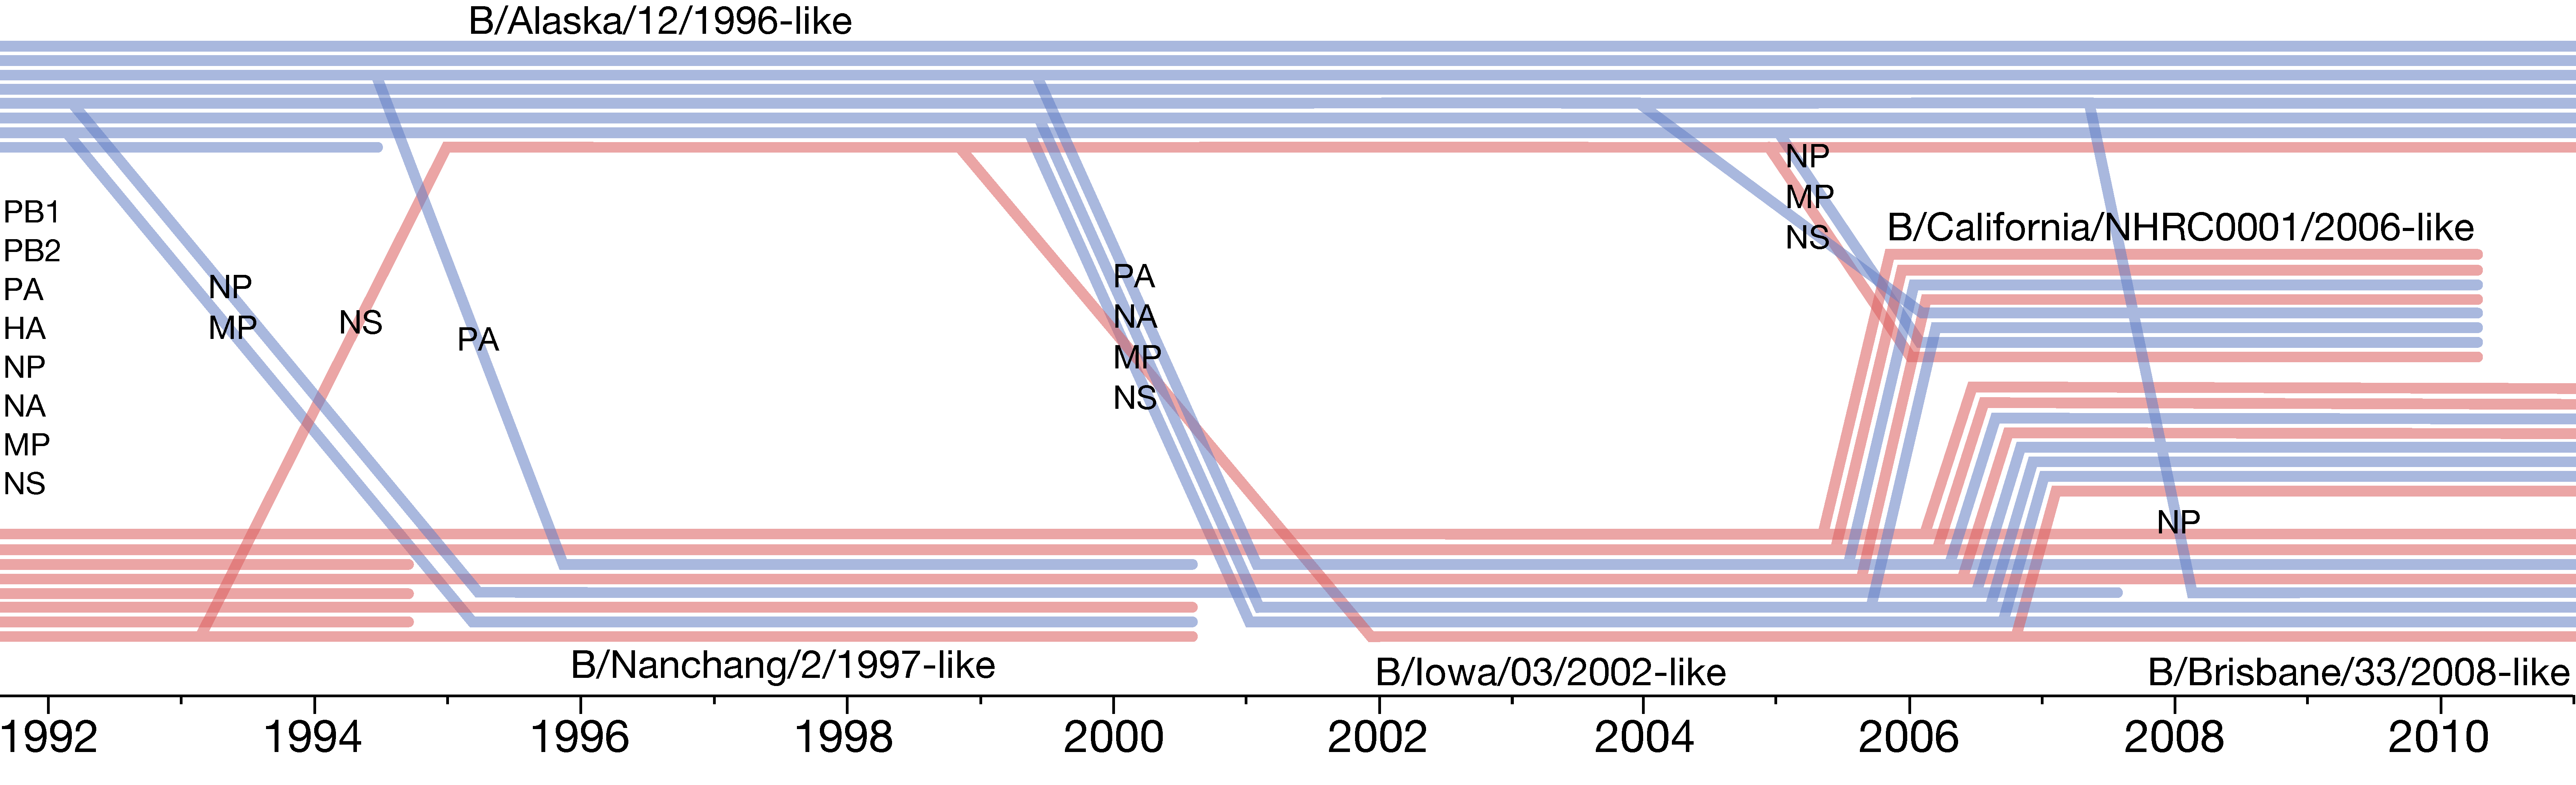
\includegraphics[width=0.95\textwidth]{figures/RailroadPlotDated.pdf}
	\caption{\textbf{Schematic plot of reconstructed reassortments between Victoria and Yamagata lineage segments of influenza B virus.}
Victoria and Yamagata lineage genomes are represented by 8 (red or blue, respectively) parallel lines.
Inter-lineage reassortment events are indicated by lines entering a different genome.
The angle of incoming lineages represents uncertainty in the timing of the event (mean date of the parent node and mean TMRCA of reassortant clades).
Lineage extinction dates are not shown accurately.}
	\label{railroadPlot}
\end{figure}



\subsection*{PB1, PB2 and HA trees experience reassortment `distance' effects}
Figure \ref{SPRdistances} shows approximate SPR distances between all pairs of trees after normalization (see Methods).
If there are biases in the way segments reassort, so that some segments tend to co-reassort more often, we expect to see small-scale similarities between phylogenetic trees of those segments.
In our case we expect SPR distances (which are proportional to the numbers of reassortment that have taken place between trees) to reflect the raw reassortment rate.
In Figure \ref{SPRdistances} the 95\% HPD intervals of normalized approximate SPR distances between pairs of segments encompass most means and occupy a relatively small range, suggesting there is no evidence of differences in the number of reassortments (or reassortment rate given as number of SPR moves per total time in the tree, data not shown) between all segments.
We note that our SPR distance analysis might simply lack power.
SPR distances themselves can only approximate (and underestimate) the actual numbers of reassortments.
In addition, we use approximate SPR distances, rather than exact SPR distances.
However, we do estimate exact SPR distances for a limited number of segment pairs (PB1-PB2 and PB1-HA) and find that after normalization exact and approximate SPR distances are not significantly different. 

Although we do not find evidence of differences in numbers of raw reassortments between all pairs of trees, we find support for a reassortment `distance' effect.
Figure \ref{deltaTMRCA} shows normalized mean $\Delta$TMRCA values for all pairs of trees.
Most segment pairs show very low values for this statistic, indicating differences in TMRCAs.
PB1, PB2 and HA trees, on the other hand, exhibit TMRCAs between themselves which are, on average, much more similar to the replicates of those trees.
This suggests that PB1, PB2 and HA lineages tend to not reassort amongst themselves unless both reassorting segments have similar TMRCAs, \textit{i.e.} there is isolation by distance.
In addition, we see evidence of a similar reassortment `distance' effect in MP and NA trees.
Previously, associations between MP and NA segments have been suspected in influenza A viruses (Samantha Lycett, personal communication).

\begin{figure}
	\centering		
	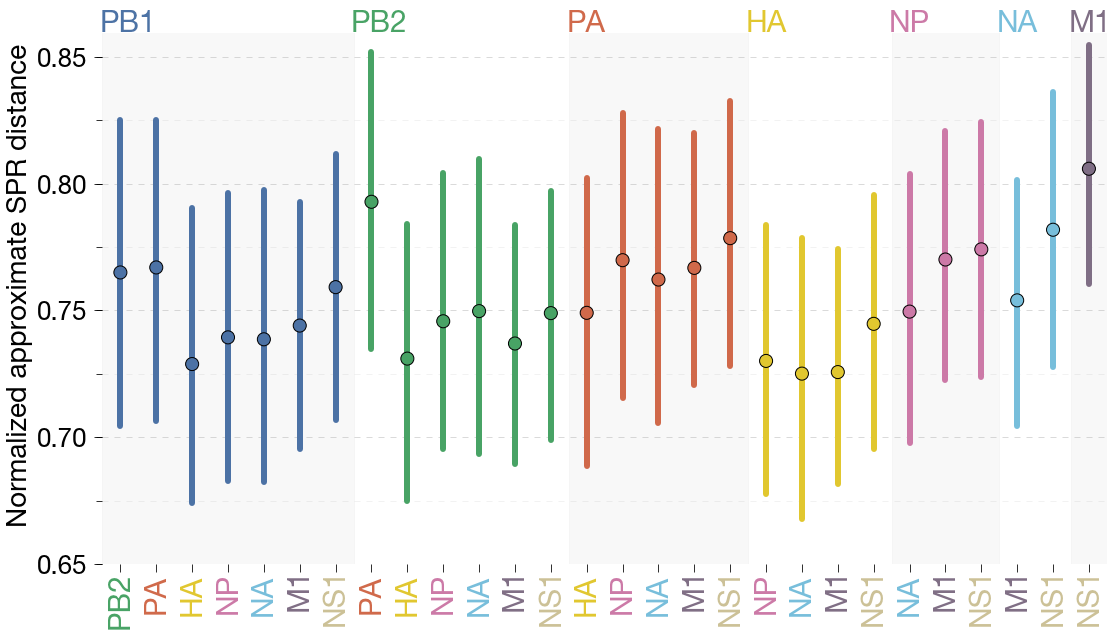
\includegraphics[width=0.95\textwidth]{figures/InfB_normalizedApproxSPR.png}
	\caption{\textbf{Normalized approximate SPR distances between pairs of segments.}
All vertical lines indicating uncertainty are 95\% highest posterior densities (HPDs).}
	\label{SPRdistances}
\end{figure}

\begin{figure}
	\centering		
	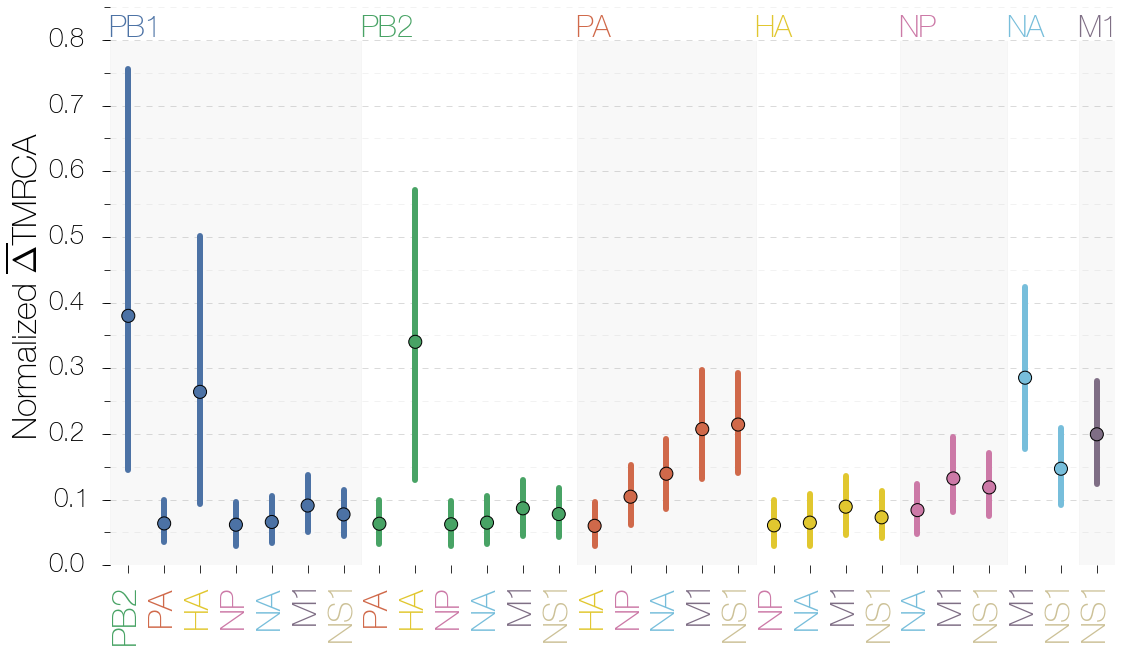
\includegraphics[width=0.95\textwidth]{figures/InfB_normalizedMuDeltaTMRCA.png}
	\caption{\textbf{Normalized mean $\Delta$TMRCA statistics between pairs of segments.}
All vertical lines indicating uncertainty are 95\% highest posterior densities (HPDs).}
	\label{deltaTMRCA}
\end{figure}

\subsection*{Linkage disequilibrium analysis confirms phylogenetic findings}
Although not an independent validation of association between PB1, PB2 and HA segments, linkage disequilibrium analyses show that Victoria and Yamagata lineages of these segments have accumulated lineage-specific amino acid substitutions.
In Figure \ref{segmentLD} their signature is greater mean $\chi^{2}_{df}$ between PB1, PB2 and HA amino acid sites than any other pair of proteins.
In some cases this value exceeds the estimated LD of amino acid sites within the same protein (\textit{e.g.} PB1 and HA).
Of the amino acid sites that exhibit high LD on PB1, PB2 and HA proteins, there are 5 sites on PB1, 8 on PB2 and 13 on HA proteins which form a network of sites exhibiting reciprocally high LD (see Supplementary information).
These sites define the split between Vic and Yam lineages within PB1, PB2 and HA segments.
In addition, there are sites on PB1, PB2 and HA proteins which also show high (albeit smaller) LD which correspond to sites which have undergone amino acid replacements some time after the Vic/Yam split.

\begin{figure}[h]
	\centering	
	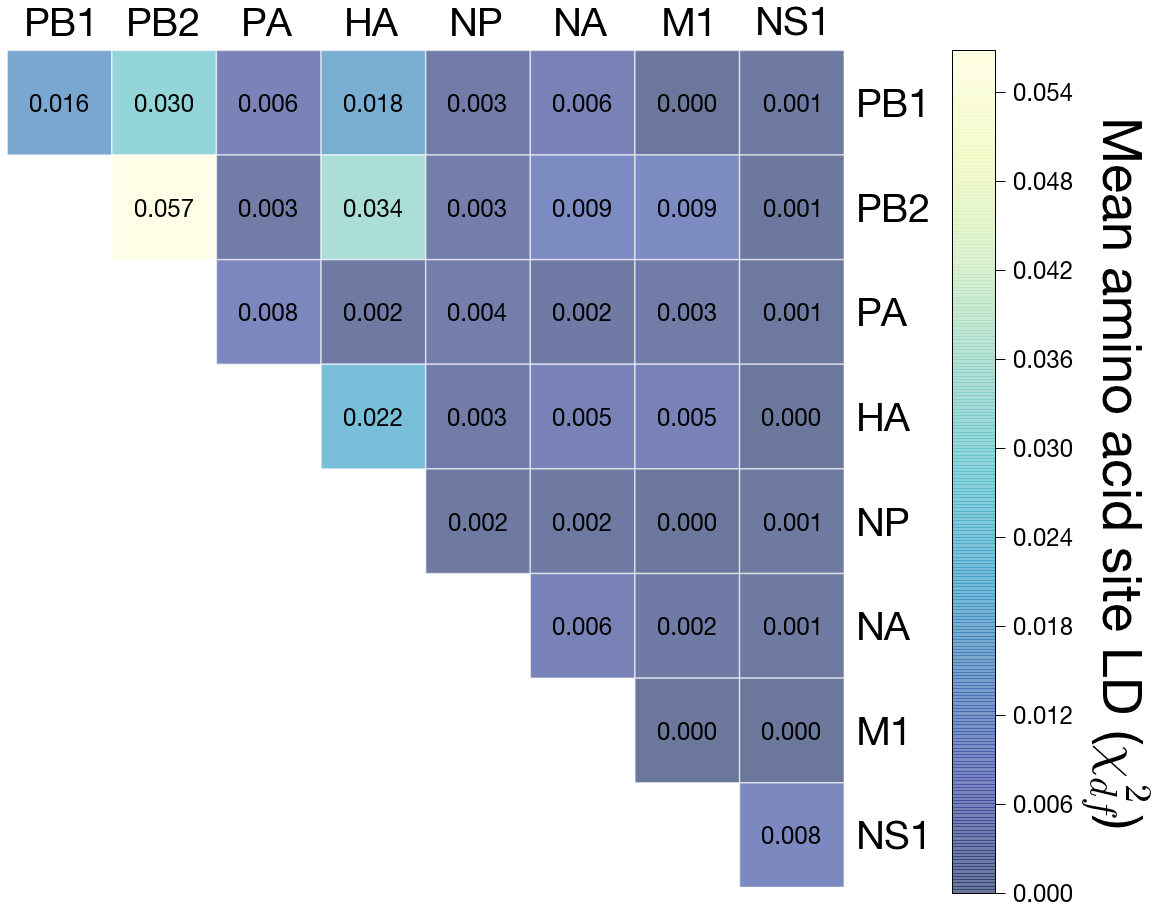
\includegraphics[width=0.75\textwidth]	{figures/InfB_aaMeanLD.png}
	\caption{\textbf{LD comparison between influenza B proteins.}
Comparison of linkage disequilibrium between amino acid sites on influenza B proteins.
Numbers on the heatmap are mean $\chi^{2}_{df}$ between pairs of proteins.}
	\label{segmentLD}
\end{figure}

\section*{Discussion}

\subsection*{Rehash streamlined version of results for people who don't read results sections.}
In this paper we have shown that PB1, PB2 and HA segments of influenza B viruses are the only ones that have maintained both a Vic and a Yam lineage (Figure \ref{lineageRatiosOverTime}).
Evidence suggests that this is a result of prolonged lack of reassortment between Vic and Yam lineages of these segments (Figure \ref{betweenDiversity}) which have evolved co-assorting amino acid sites detectable as high linkage disequilibrium (Figure \ref{segmentLD}).
We propose that this pattern of non-reassortment is due to the action of selection and not simply biased reassortment.
Figures \ref{SPRdistances} and \ref{deltaTMRCA} show that despite all pairs of segments having the same reassortment frequency, PB1, PB2 and HA segments exhibit much lower reassortment `distances'.
Reassortment `distances' represent the temporal separation of reassorting lineages and suggests that reassortments between PB1, PB2 and HA segments tend to combine lineages that have relatively recently been part of the same genome (\textit{i.e.} that have shared a recent common virion).
In addition, most strains with mixed-lineage PB1-PB2-HA complexes occured in the early years of the Vic--Yam split, when the two lineages were much more similar at the nucleotide and amino acid levels.
The most recent lineage of influenza B viruses with mixed-lineage PB1-PB2-HA complexes (B/Waikato/6/2005-like) only circulated for 5 months before going extinct.
We suggest that the preservation of two PB1-PB2-HA complex lineages is similar to genomic speciation islands \textit{i.e.} small numbers of genes that resist being homogenized through gene flow.
Thus, if both PB1-PB2-HA complex lineages continue circulating in humans we expect more segments to be recruited to the two complexes, resulting in eventual sympatric speciation of influenza B viruses. 
\tbc{Title is approximate.}

\subsection*{Potential causes of co-dependence between PB1-PB2-HA}
Previous studies have investigated possible co-dependence patterns between segments of influenza B viruses, by focusing on segments which would be expected to be co-adapted, \textit{e.g.} PB1-PB2-PA and HA-NA \cite{mccullers2004}.
Though it would be easy to explain co-adaptation between the aforementioned segments by referring to their functional roles (\textit{e.g.} PB1-PB2-PA form the polymerase heterotrimer and HA-NA have antagonistic activities), our findings suggest a counter-intuitive relationship between PB1, PB2 and HA segments.

It is clear that PB1-PB2-HA segments of Vic and Yam lineages do not preferentially reassort together: there have been at least 4 sampled mixed-lineage PB1-PB2-HA complex constellations (which did not become fixed in the population) and our estimates of the number of reassortments do not differ significantly between all segments.
Figure \ref{SPRdistances} and recent evidence suggests that, at least in influenza A, reassortment between segments differing by a single synonymous difference is highly efficient \cite{marshall2013}.
In the absence of clear functional explanations for why PB1, PB2 and HA should be co-adapted we suggest several alternatives.

It is perhaps easiest to explain co-dependence between PB1 and PB2 segments based on their functions as part of the influenza RNA-dependent RNA polymerase (RdRp) heterotrimer.
Indeed, trees of PB1 and PB2 segments exhibit high similarity in tip--tip TMRCAs (Figure \ref{deltaTMRCA}), suggesting highly similar TMRCAs.
In addition, PB1--PB2 reassortants are the rarest and least persistent amongst mixed-lineage PB1-PB2-HA strains and have not been isolated since 1996.

Explaining the co-dependence between PB1+2 and HA segments is more difficult.

Many studies have noted a possible link between the HA, NA and PB1 segments of influenza A viruses \cite{bergeron2010,fulvini2011}.
Early influenza A vaccines used to be derived by infecting chicken eggs with an egg-adapted strain and a seasonal human isolate in the presence of antisera raised against the HA and NA proteins of the egg-adapted strain, thus selecting for reassortants which were egg-adapted (\textit{i.e.} had internal segments derived from the egg-adapted strain) but possessed the HA and NA segments of the seasonal strain.
However, in addition to producing reassortants with HA-NA derived from the seasonal strain, as intended, the second most frequent class of reassortants produced using this methods were those with PB1, HA and NA derived from seasonal strains \cite{bergeron2010,fulvini2011}.

Recent experiments have suggested that the presence or absence of a `foreign' PB1 segment can have dramatic effects on HA concentration on the surface of virions and total virion production \cite{cobbin2013}.
Additional evidence for a relationship between PB1 and HA segments in influenza A viruses is given by previous influenza pandemics, which were caused by avian-human influenza A virus reassortants.
It has been established that at least for the 1957 and the 1968 influenza pandemics, caused by A/H2N2 and A/H3N2 subtypes, respectively, the viruses responsible were reassortants possessing PB1 and HA segments (and in the case of A/H2N2, NA as well) derived from avian influenza A viruses \cite{kawaoka1989}.
However, there have also been reassortant influenza viruses circulating for prolonged periods of time in humans that did have disparate PB1 and HA segments, \textit{e.g.} H1N2 outbreaks in 2001 \cite{gregory2002} and H1N1/09 in 2009 \cite{smith2009}.


Another possibility is the action of balancing selection in preserving the diversity in one segment, whilst the other segments hitchhike along.
A good candidate for this would be HA, as it is now the sole bearer of antigenic diversity within the influenza B population (the Vic lineage NA segment having gone extinct in 2002 (Figures \ref{tmrcaOT} and \ref{railroadPlot})), until the Yam lineage NA segment under Vic PB1-PB2-HA recovers sufficient antigenic diversity.
Previous research has found that avian influenza A virus HA and NA segments, which are the primary vehicles of antigenicity, exhibit vast diversity when compared to `internal segments', which show much more recent TMRCAs and less variability at the amino acid level \cite{chen2006,obenauer2006}.
This is easiest to interpret as frequency-dependent balancing selection acting to preserve antigenic diversity.
If this is the case in influenza B viruses, we expect balancing selection to act on HA and indirectly, through some unknown association with HA, on PB1 and PB2 segments.
It is also possible that Vic and Yam lineages of PB1, PB2 and HA segments have simply drifted away from each other, without any one segment being the driver of diversity preservation in PB1, PB2 and HA segments.
This process, termed mutation-driven co-evolution \cite{presgraves2010}, has been suggested to be the cause of hybrid dysfunction in \textit{Saccharomyces} hybrids \cite{lee2008}.

Finally it is possible that PB1 and PB2 segments are co-adapted whereas the HA segment is simply hitchhiking along stochastically. 
We find it unlikely given that B/Waikato/6/2005-like strains, the most recent isolates with a mixed-lineage PB1-PB2-HA complex, circulated for a limited amount of time within a limited geographic area, suggesting that this particular lineage was outcompeted by influenza B strains with `pure' PB1-PB2-HA complexes.

\subsection*{The future of influenza B viruses}
We see three potential paths of evolution for influenza B viruses.
More segments could be recruited into the two currently circulating co-adapted segment complexes (PB1, PB2 and HA segments being the genomic speciation islands), as part of a speciation process, until all circulating influenza B viruses possess genomes with segments firmly associated with either the Vic or Yam lineage PB1-PB2-HA complex which could be referred to as belonging to either `new Victoria' or `new Yamagata' lineages.

Sympatric speciation in other systems usually requires strong barriers to introgression, \textit{e.g.} infertility of F1 hybrids can lead to the evolution of prezygotic reproductive isolation otherwise known as reinforcement or Wallace effect.
To what extent this would apply to influenza B viruses remains unknown.

If influenza B viruses are undergoing sympatric speciation, does co-infection with Victoria and Yamagata lineages of PB1-PB2-HA segments occur at a sufficiently high frequency and result in considerable losses of fitness to drive the evolution of reassortment isolation mechanisms (\textit{e.g.} unique packaging signals) or is co-infection so rare that speciation occurs via mutation-driven co-evolution?
Given that PB1 and PB2 segments are functionally linked, is it reasonable to expect that the next segment to be recruited to the PB1-PB2-HA segment complexes will be functionally linked to either PB1/PB2 or HA?

Are the reassortment events of the past 20 years (Figure \ref{railroadPlot}) which frequently involved the NP, MP and NS segments from a Yamagata PB1-PB2-HA background entering a Victoria PB1-PB2-HA background via reassortment indicative of rare events followed by selective sweeps or stochastic fixation?

It's not unfeasible for selective sweeps following reassortments to breakdown developing co-adaptation of segments, especially if they are not functionally linked and have themselves been reassorted into a new PB1-PB2-HA background recently.
This is the second scenario we might expect to occur, whereby relatively frequent reassortments occur between Vic and Yam lineages and are followed by selective sweeps.
In this case influenza B viruses would undergo periodic genome homogenization with the exception of PB1, PB2 and HA segments.
However, this model would require strong selective sweeps and/or relatively frequent reassortments, neither of which seem to be lacking in the influenza B virus population.

Given the relatively recent explosion of sequence data available for influenza B, it is difficult to say whether dynamics similar to Victoria and Yamagata lineages have not occurred in influenza B virus genomes before and left no trace through extinction.
We find it unlikely that either Victoria or Yamagata lineage PB1-PB2-HA complexes will go extinct stochastically in the near future, as they have co-circulated for prolonged periods at a ratio close to 0.5, suggesting the action of balancing selection (Figure \ref{lineageRatiosOverTime}).
Depletion of susceptible individuals through influenza pandemics or vaccination seem unlikely as well.
Both Victoria and Yamagata lineage PB1-PB2-HA complexes survived the admittedly mild influenza pandemic in 2009 and influenza vaccines do not produce lifelong immunity.


\subsection*{Predictions}
Using previously developed plasmid systems \cite{hoffmann2002} it would be possible to create artificial reassortants, combining Vic and Yam lineages of PB1, PB2 and HA segments into mixed-lineage PB1-PB2-HA complexes.
We predict that artificially produced viruses with mixed-lineage PB1-PB2-HA complexes will have reduced fitness when compared to viruses with pure-lineage (\textit{i.e.} entirely Vic or entirely Yam) PB1-PB2-HA complexes.
In addition, we expect the relationship between Vic and Yam lineage PB1, PB2 and HA segments to be dependent on date of segment isolation, as viruses with mixed-lineage PB1-PB2-HA complexes isolated earlier should perform better than viruses with PB1-PB2-HA segments isolated more recently.

Given the existence of B/Waikato/6/2005-like viruses and the rarity of PB1-PB2 reassortants we expect that artificially produced PB1-PB2 reassortants would be much less fit than either PB1-HA or PB2-HA reassortants.

However, we also see that epistatic effects might interfere with fitness measurements, if for example non-PB1-PB2-HA segments are also temporally mismatched.
Ideally, the co-adaptation would be easier to understand by referring to the structures of PB1 and PB2 proteins, as the link between these would be intuitive.
We have identified amino acid sites which are linked between PB1, PB2 and HA proteins of Victoria and Yamagata lineages, but we find very few sites on PB1 and PB2 proteins that fall within the regions that form contacts within the influenza B polymerase heterotrimer, suggesting more subtle roles for sites we have identified.

\subsection*{Implications for influenza B virus control and prevention}
It is our hope that understanding the mechanism(s) underlying the links between Vic and Yam lineage PB1-PB2-HA complexes might suggest a more varied approach to both influenza B surveillance and control.
For one, our findings suggest that viruses bearing mixed-lineage PB1-PB2-HA complexes, if unveiled by surveillance, are unlikely to contribute to future influenza B evolution (as seen with B/Waikato/6/2005-like viruses).
Similarly, in the absence of sequence data, it should be possible to predict the lineage of PB1, PB2 and HA segments of influenza B viruses by sequencing only one of those segments.

It remains to be seen whether equivalent or similar links exist between segments of influenza A viruses, which present a much greater threat to human health worldwide than influenza B viruses.
By discovering the underlying mechanism by which PB1, PB2 and HA are co-adapted might reveal potential targets for new classes of antiviral drugs.

\section*{Conclusions}
In this study we have investigated the patterns of reassortment amongst two influenza B virus segment lineages and found preserved diversity and consistent co-reassortment of 3 segments: PB1, PB2 and HA.
Our findings reveal that Vic and Yam lineages of PB1, PB2 and HA segments co-associate amongst themselves with segments of their own lineage, thus resulting in an entirely Vic-lineage-derived PB1-PB2-HA segment complex and an entirely Yam-lineage-derived PB1-PB2-HA segment complex that co-circulate within the influenza B virus population, occasionally exchanging non-PB1-PB2-HA segments.
Though we detect strains with mixed-lineage PB1-PB2-HA complexes, we find that they have performed poorly and have circulated for short amounts of evolutionary time when compared to viruses with `pure' lineage PB1-PB2-HA complexes.

We argue that this is evidence for a selectively maintained relationship between PB1-PB2-HA complex of Vic and Yam lineages and not due to biased reassortment.
Given sufficient time we expect the two PB1-PB2-HA complexes to recruit the rest of the genomic segments into co-adapted and co-reassorting segment complexes eventually resulting in sympatric speciation of influenza B viruses.


%\begin{figure}[h]
%	\centering		
%	\includegraphics[width=0.95\textwidth]{figures/InfB_TMRCAOverTime}
%	\caption{\textbf{Provisional TMRCA over time plot.}}
%\end{figure}


\bibliographystyle{pnas}
\bibliography{fluB}
\end{document}
